

\begin{subsubsection}{Diseño de la red del SDDC con VMware NSX-T}
    En el SDDC existe una red virtual que se define mediante software, también se le llama Software Defined Network (SDN). Esta red virtual está desacoplada de la infraestructura física, lo cual permite modificar su configuración sin necesidad de realizar cambios en la infraestructura de red ni en la configuración de los dispositivos de red físicos. Además, al estar definida por software, permite implementar diferentes configuraciones de red, mejorando y simplificando la administración y seguridad de las nuevas redes que se añaden al entorno. El componente encargado de mantener las redes virtuales del SDDC es VMware NSX-T.

    
    % proporcionando elasticidad y flexibilidad a la hora de administrar y obtener los recursos, tanto para el administrador como para el usuario final. 
    En el Management Domain se despliega una instancia de NSX-T Manager y dos instancias del componente NSX-T Edge.
    % Para mantener la disponibilidad de VMware NSX-T y balancear su carga de trabajo, se despliegan tres instancias de NSX-T Manager Appliance, aunque para reducir el consumo de recursos, en el entorno de prueba solo se creará una instancia de este componente llamada \textit{nsx-mgmt-1}. También se despliegan dos instancias del componente VMware NSX-T Edge, llamadas \textit{edge01-mgmt} y \textit{edge02-mgmt}.

    La virtualización de la red con VMware NSX-T se basa en dos componentes, Transport Zone (TZ) y Segment.
    \begin{itemize}
        \item Transport Zone: se trata de un contenedor dentro del cual se definen Segments. A una TZ se conectan TNs\footnote{Los Transport Nodes son los hosts físicos y cada instancia de VMware NSX-T Edge.} para acceder a los Segments. Cada TN puede estar conectado a varias Transport Zones.
        \item Segment: se trata de un dominio de broadcast de capa 2, es decir, una subred, que forma parte de una TZ. Las VMs se conectan a los Segments que pertenecientes a cada TZ.
    \end{itemize}
    Una TZ se extiende en diferentes hosts que pueden estar situados tanto en la misma red a nivel físico, como en distintas partes de la infraestructura del SDDC. Los hosts que estén conectados a una TZ tendrán acceso a los Segments, es decir, subredes, que esta contenga. Así, se hace posible la creación de redes accesibles desde cualquier parte de la infraestructura del SDDC sin necesidad de modificar los dispositivos de red físicos.
    En el entorno, existen dos TZs. Una de ellas, la TZ \textit{mgmt-domain-m01-overlay-tz}, contiene dos Segments, \textit{mgmt-Region01A-VXLAN} y \textit{mgmt-xRegion01-VXLAN}, los cuales son utilizados para conectar las instancias de los componentes de VMware vRealize Suite. La otra TZ disponible, \textit{sfo01-m01-edge-uplink-tz} contiene otros dos Segments, utilizados para dar salida hacia el router VyOS al tráfico que circula por la TZ anterior (\textit{mgmt-domain-m01-overlay-tz}). Para que el tráfico de cada Segment pueda circular por la red física de la infraestructura, VMware NSX-T lo encapsula cuando sale del host para que este pueda llegar al host destinatario.
    Los encargados de gestionar el enrutamiento entre Segments y hacia la red externa son las instancias de NSX-T Edge. Para ello, internamente forman una estructura de routers virtuales que a parte de realizar las tareas de enrutamiento, proporcionan servicios de red como NAT, Load Balancing, DNS, DHCP, VPN y Firewall, y mantienen rutas redundantes hacia el dispositivo físico de red.
    \begin{figure}[h]
        \centering
        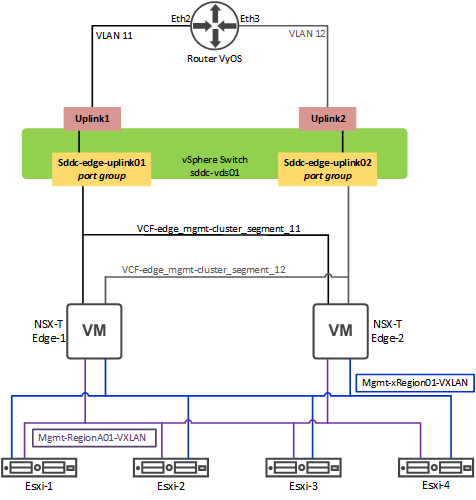
\includegraphics[width=0.8\textwidth]{imaxes/pruebaconcepto/estructura_NSX_T.png}
        \caption{Conexiones mantenidas por los nodos que forman parte de NSX-T para establecer redes virtuales.}
        \label{fig:estructura-NSXT}
      \end{figure}
      \FloatBarrier

    \begin{figure}[h]
        \centering
        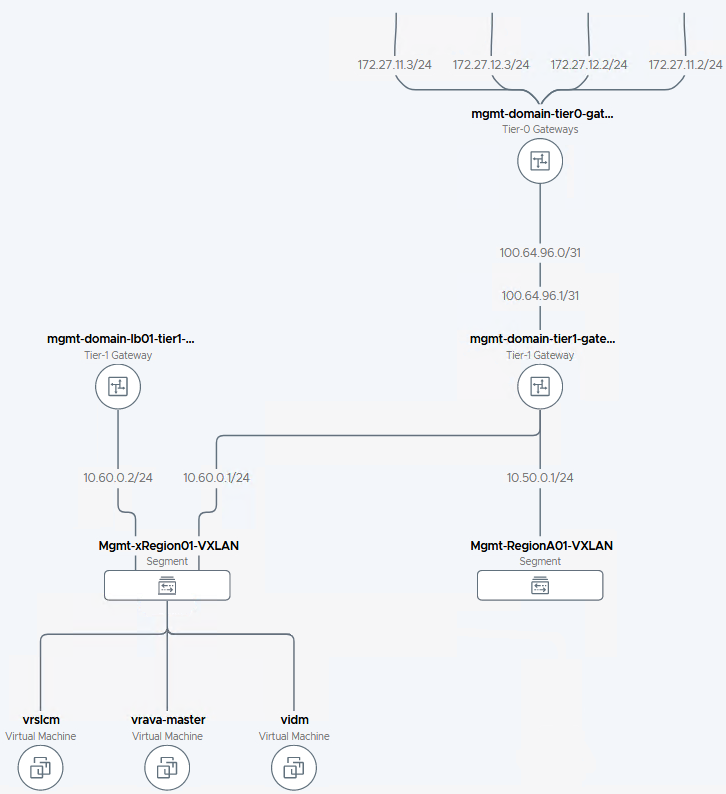
\includegraphics[width=0.6\textwidth]{imaxes/pruebaconcepto/topologiaTwoTierRouting-Final.png}
        \caption{Topología virtual de VMware NSX-T}
        \label{fig:two-tier-topology} 
    \end{figure}
    \FloatBarrier

    En la primera imagen (Figura \ref{fig:estructura-NSXT}), se muestra como cada nodo se conecta a los Segments disponibles para que las VMs que se residen en ellos puedan acceder a la red. Como ya se ha comentado, las VMs de NSX-T Edge enrutan el tráfico hacia la red física a través del vDS desplegado en VMware vSphere. En la segunda imagen (Figura \ref{fig:two-tier-topology}), se muestra la misma estructura pero desde el punto de vista interno de VMware NSX-T. En ella se aprecian los dos Segments donde uno de ellos tiene tres VMs conectadas (componentes de VMware vRealize Suite), y tres routers virtuales (dos Tier-1 y un Tier-0). Los routers Tier-1 proporcionan servicios de red, \textit{mgmt-domain-lb01-tier1} proporciona un balanceador de carga para los componentes de VMware vRealize Suite, y enrutamiento entre Segments, mientras que el router Tier-0 se encarga de de dirigir el tráfico hacia la red física (router VyOS) a través de cuatro conexiones que se corresponden con las que se conectan al vDS que se muestra en la imagen anterior (Figura \ref{fig:estructura-NSXT}). Para que el router VyOS tenga conocimiento de las redes virtuales de VMware NSX-T, las instancias de NSX-T las anuncian con el protocolo de enrutamiento dinámico BGP.
    \\
    Usando VMware NSX-T, el administrador puede gestionar y crear redes para ser consumidas por los usuarios de la plataforma. La creación de estas redes virtuales se hace bajo demanda y no requiere ninguna configuración adicional en los dispositivos de la red física. Su gestión se realiza siempre desde VMware NSX-T, el cual permite monitorizarlas, controlar su seguridad y establecer servicios dedicados a estas redes virtuales. Además, permite extender una red virtual sobre diferentes redes físicas permitiendo acceder a las VMs conectadas a ella desde diferentes puntos y permitir migraciones de VMs de una localización a otra sin necesidad de cambiar la configuración, ni de la VM ni de la red física. En la infraestructura actual del CITIC todo esto no es posible, las redes que se crean dentro del entorno de VCF deben configurarse previamente sobre la red física, y todos los servicios de red necesarios deben ser proporcionados también desde dispositivos físicos, es decir, no existe una plataforma que permita gestionar las redes de la infraestructura de una forma dinámica y sin un alto coste en tiempo y riesgos.
    
    
    % VMware NSX-T se encarga de encapsular el tráfico de estas redes virtuales 
    
    % Cuando el tráfico de un Segment debe salir de un TN a la red física para alcanzar su destino\footnote{Este paquete contiene la información de las VMs origen y destino que se están comunicando.}, este es encapsulado de nuevo en un paquete con la información de los TN origen y destino[Fig. \ref{fig:Frame-Segment-NSXT}]. Gracias a esta encapsulación, elementos que se encuentran en distintos entornos de la red física se pueden comunicar como si estuvieran directamente conectados el uno al otro. Así, es posible la creación de una misma red que se extienda por toda la infraestructura del SDDC, permitiendo comunicar componentes situados en distintas redes físicas, sin necesidad de modificar la configuración de los dispositivos físicos ni su topología. Esto hace necesario el uso de un protocolo de enrutamiento dinámico con BGP, tanto en la infraestructura física como en la red virtual, y así automatizar el proceso de configuración de nuevas redes virtuales.
    % El tipo de encapsulación que se realiza sobre el tráfico de los Segments se define la configuración de cada TZ, esta puede  ser de tipo VLAN o de tipo Overlay usando el protocolo Geneve.
    % \begin{itemize}
    %     \item TZ de tipo VLAN: se define una VLAN que se utilizará para identificar y encapsular el tráfico perteneciente a los Segments de una misma TZ. La VLAN que se defina debe estar configurada en la red física para que su tráfico sea aceptado.
    %     \item TZ de tipo Overlay Geneve: este protocolo se encarga de encapsular el tráfico saliente añadiendo una cabecera extra donde incluye un identificador. Cada Segment tendría su propio identificador.
    % \end{itemize}
    % \begin{figure}[h]
    %     \centering
    %     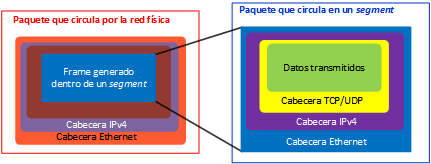
\includegraphics[width=0.8\textwidth]{imaxes/pruebaconcepto/Frame.png}
    %     \caption{Paquete de un Segment encapsulado cuando sale a la red física.}
    %     \label{fig:Frame-Segment-NSXT}
    % \end{figure}
    % \FloatBarrier
    % En la imagen anterior se muestra como se encapsula un paquete perteneciente a un Segment cuando este sale de un host/TN al medio físico. En las cabeceras del paquete correspondiente al Segment tendrá la información sobre las VMs origen y destino que se están comunicando, mientras que las cabeceras que encapsulan a ese paquete contienen la información sobre los hosts/TNs origen y destino donde se encuentran las VMs que se están comunicando. La dirección IP utilizada por los hosts/TNs para enviar el tráfico de un Segment encapsulado, se denomina Tunnel End-Point (TEP) y se asigna mediante DHCP para automatizar su configuración cuando un nuevo host/TN es añadido al entorno.

    % \begin{figure}[h]
    %     \centering
    %     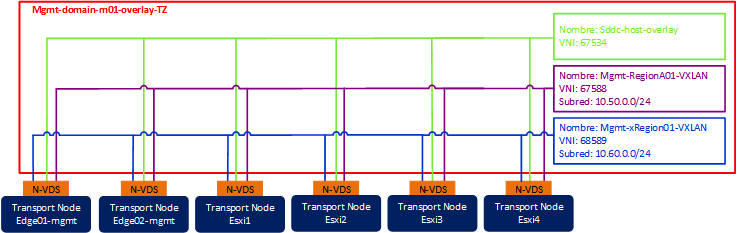
\includegraphics[width=0.8\textwidth]{imaxes/pruebaconcepto/OverlayTZSegments.png}
    %     \caption{Segments de la Transport Zone \textit{mgmt-domain-m01-overlay-tz}}
    %     \label{fig:overlay-TZ-segments-NSXT}
    %   \end{figure}
    %   \FloatBarrier

    %   En la imagen anterior se muestra la Transport Zone de tipo Overlay, definida en el entorno de pruebas, con el nombre \textit{mgmt-domain-m01-overlay-tz}. A ella se conectan los seis TNs\footnote{Los seis TNs son los cuatro hosts y las dos instancias de NSX-T Edge}\footnote{Un TN utiliza el elemento NSX-T Virtual Distributed Switch (N-VDS) para conectarse a los Segments de una TZ} y contiene tres Segments. El Segment \textit{mgmt-xRegion01-VXLAN} se utiliza para desplegar aplicaciones cuyas instancias deben ser accesibles desde cada Region del SDDC. El Segment \textit{mgmt-Region01A-VXLAN} tiene como finalidad alojar aplicaciones que solo deben ser accesibles desde dentro de una misma Region. El Segment \textit{sddc-host-overlay} es utilizado por los componentes de VMware NSX-T para comunicarse con los TNs. Con cada Segment de tipo Overlay se genera un \textit{port group} con el mismo nombre en el vDS (se puede ver en la figura \ref{fig:port-groups-vSwitch-vSphere}) que se utilizan para transmitir su tráfico a la red física.
    % %    VMware NSX-T genera en el vSphere vSwitch un \textit{port group} por cada \textit{segment} para poder conectar la VM de cada componente al \textit{port group} que le corresponda.

    % \begin{figure}[h]
    %     \centering
    %     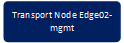
\includegraphics[width=0.8\textwidth]{imaxes/pruebaconcepto/VLANTZSegments.png}
    %      \caption{Segments de la  Transport Zone \textit{sfo01-m01-edge-uplink-tz}}
    %     \label{fig:VLAN-TZ-segments-NSXT}
    % \end{figure}
    % \FloatBarrier
    % En la imagen anterior se muestra la Transport Zone de tipo VLAN, definida en el entorno de pruebas, con el nombre \textit{sfo01-m01-edge-uplink-tz}. A ella se conectan los dos TNs que son instancias de NSX-T Edge, \textit{edge01-mgmt} y \textit{edge02-mgmt}. Contiene dos Segments, \textit{VCF-edge-mgmt-cluster-segment-11} y \textit{VCF-edge-mgmt-cluster-segment-12}, que son utilizados por las instancias de NSX-T Edge para transmitir el tráfico de todas las redes virtuales gestionadas por VMware NSX-T hacia redes físicas externas al SDDC. Para ello utilizan utilizan los \textit{port groups} \textit{sddc-edge-uplink01} y \textit{sddc-edge-uplink02} (se pueden ver en la figura \ref{fig:port-groups-vSwitch-vSphere}) del vDS para transmitir su tráfico hacia las interfaces de red físicas de cada host. Ambas instancias forman la topología de red, que se muestra en la siguiente imagen, para comunicar las redes virtuales de VMware NSX-T con el router físico.
    % \begin{figure}[h]
    %     \centering
    %     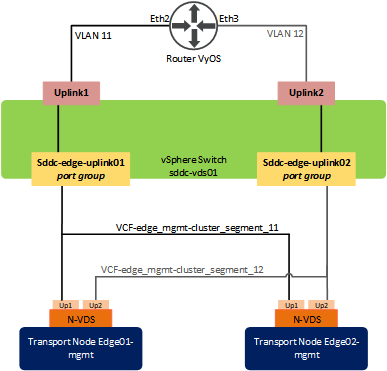
\includegraphics[width=0.4\textwidth]{imaxes/pruebaconcepto/UplinkDesign.png}
    %     \caption{Topología de red de las insterfaces \textit{uplink}.}
    %     \label{fig:Uplink-Design-Edge-NSXT} 
    % \end{figure}
    % \FloatBarrier
    % Como se puede ver en la imagen anterior, los dos Segments son utilizados por las instancias de NSX-T Edge para mantener rutas redundantes hacia la red externa y así aumentar su disponibilidad. A parte, este componente también se encarga de proporcionar un conjunto de servicios de red a los componentes que están conectados a los Segments de VMware NSX-T. Para entregar estos servicios, internamente, VMware NSX-T forma una topología con una serie de routers virtuales.
    % \begin{figure}[h]
    %     \centering
    %     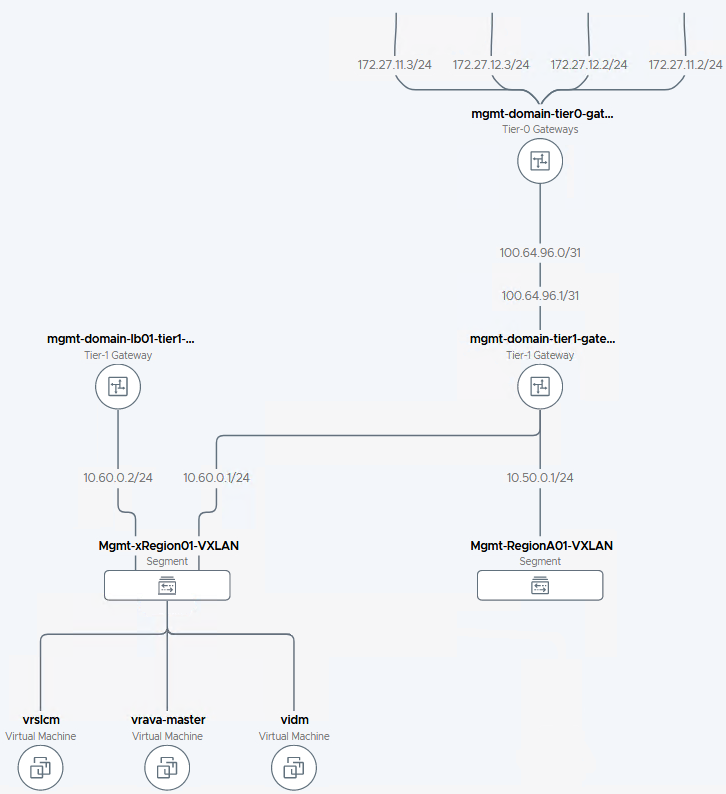
\includegraphics[width=0.4\textwidth]{imaxes/pruebaconcepto/topologiaTwoTierRouting-Final.png}
    %     \caption{Topología virtual de VMware NSX-T}
    %     \label{fig:two-tier-topology} 
    % \end{figure}
    % \FloatBarrier
    % En la imagen anterior se muestra la topología que forman VMware NSX-T para proporcionar acceso a la red externa y para entregar otros servicios a los componentes situados en los dos Segments existentes. En esta topología hay tres routers, \textit{mgmt-domain-tier0-gateway}, \textit{mgmt-domain-tier1-gateway} y \textit{mgmt-domain-lb01-tier1-gateway}, de los cuales, el primero se encarga de gestionar la comunicación con los dispositivos de red físicos, y los dos restantes se encargan de enrutar el tráfico entre Segments y hacia el router de Tier 0, y de entregar distintos servicios a los componentes que residen en los Segments. Los servicios de red que se pueden habilitar en los dos routers de Tier 1 son NAT, Load Balancing, DNS y VPN.
\end{subsubsection}